\documentclass{article}

\usepackage[brazilian]{babel}
\usepackage[utf8]{inputenc}
\usepackage[T1]{fontenc}
\usepackage{amsmath}
\usepackage{MnSymbol}
\usepackage{wasysym}
\usepackage{mdframed}
\usepackage[a4paper, total={6in, 10.5in}]{geometry}
\usepackage{graphicx}
\graphicspath{ {baciasNewton/} }

\title{MAC0210 - Laboratório de Métodos Numéricos}
\author{Exercício-programa 1}
\date{ }


\begin{document}

\maketitle

\begin{center}
\large{Vítor Kei Taira Tamada - 8516250}

\large{André Ferrari Moukarzel - 9298166}
\end{center}

\section{Parte 1: Aritmética de ponto flutuante}

\textbf{Questão 1 (3.11): Dado o sistema de ponto flutuante com base 2:}
\begin{center}
$x = \pm S \times 2^{E}$

sendo que

$S = (0.1b_{2}b_{3}b_{4}...)$

$-128 < E < 127$
\end{center}

\quad\textbf{a) Qual é o maior número de ponto flutuante desse sistema?}

\bigskip
\qquad R) O maior número de ponto flutuante que esse sistema é capaz de representar é:
\begin{center}
$+(0.111111111111111111111111) \times 2^{126}$
\end{center}

\qquad que é equivalente a

\begin{center}
$+111111111111111111111111 \times 2^{102}$
\end{center}

\qquad Como $111111111111111111111111$ equivale a $16777215$ em base $10$, temos que o maior número que esse sistema consegue representar é:

\begin{center}
$16777215 \times 2^{102}$
\end{center}

\quad\textbf{b) Qual é o menor número de ponto flutuante positivo desse sistema?}

\bigskip
\qquad R) O menor número de ponto flutuante positivo que esse sistema é capaz de representar é:

\begin{center}
$+(0.100000000000000000000000) \times 2^{-127}$
\end{center}

\qquad Como $0.100000000000000000000000$ equivale a $0.5$ em base $10$, temos que o menor número positivo que esse sistema consegue representar é:

\begin{center}
$0.5 \times 2^{-127}$
\end{center} 

\quad\textbf{c) Qual é o menor inteiro positivo que não é exatamente representável nesse sistema?}

\bigskip
\qquad R) O menor número positivo não representável no sistema é o número com o menor S dentro do intervalo e o menor E acima do intervalo. Ou seja,

\begin{center}
$S = 0.100000000000000000000000$

$E = 127$
\end{center}

\qquad Logo, o menor inteiro não representável nesse sistema é o

\begin{center}
$x = 0.5 \times 2^{127}$
\end{center}

\begin{flushright}
$\blacksquare$
\end{flushright}

\textbf{Questão 2 (5.1): Qual é a representação do número $\frac{1}{10}$ no formato IEEE single para cada um dos quatro modos de arredondamento? E para os números $1 + 2^{-25}$ e $2^{130}$?}

\bigskip
\quad R) As representações no formato IEEE single em cada um dos quatro modos de arredondamento são as seguinte:

\bigskip
\qquad [Para $\frac{1}{10}$]

\qquad$\bullet$ Aproximação para $+\infty$:

\qquad\qquad$(0.00011001100110011001101)_{2} \times 2^{0}$

\bigskip
\qquad$\bullet$ Aproximação para $-\infty$:

\qquad\qquad$(0.00011001100110011001100)_{2} \times 2^{0}$

\bigskip
\qquad$\bullet$ Aproximação para $0$:

\qquad\qquad$(0.00011001100110011001100)_{2} \times 2^{0}$

\bigskip
\qquad$\bullet$ Aproximação para o mais próximo:

\qquad\qquad$(0.00011001100110011001101)_{2} \times 2^{0}$

\bigskip\bigskip
\qquad [Para $1 + 2^{-25}$, sabendo que a mantissa tem 23 bits]

\qquad$\bullet$ Aproximação para $+\infty$:

\qquad\qquad$(0.10000000000000000000001)_{2} \times 2^{1}$

\bigskip
\qquad$\bullet$ Aproximação para $-\infty$:

\qquad\qquad$(0.10000000000000000000000)_{2} \times 2^{1}$

\bigskip
\qquad$\bullet$ Aproximação para $0$:

\qquad\qquad$(0.10000000000000000000000)_{2} \times 2^{1}$

\bigskip
\qquad$\bullet$ Aproximação para o mais próximo:

\qquad\qquad$(0.10000000000000000000000)_{2} \times 2^{1}$

\bigskip\bigskip
\qquad [Para $2^{130}$]

\qquad\emph{Uma vez que o formato IEEE single não consegue representar números maior do que $2^{128}$ (sendo que esse limite é reservado para representar $\infty$), o número $2^{130}$ não possui aproximação nesse sistema}

\begin{flushright}
$\blacksquare$
\end{flushright}

\bigskip
\textbf{Questão 3 (6.4): Qual é o maior número de ponto flutuante $x$ tal que $1 \oplus x$ é exatamente 1, assumindo que o formato usado é IEEE single e modo de arredondamento para o mais próximo? E se o formato for IEEE double?}

\bigskip
\quad R) Dada uma mantissa binária com $t$ bits de precisão, um número $x \leqslant 2^{-(t+2)}$  é arredondado para baixo se utilizar arredondamento para mais próximo. Portanto, o número $x$ é:

\bigskip
\qquad$\bullet$ Para IEEE single, $2^{-25}$

\qquad$\bullet$ Para IEEE double, $2^{-54}$

\begin{flushright}
$\blacksquare$
\end{flushright}

\bigskip
\textbf{Questão 4 (6.8): Em aritmética exata, a soma é um operador comutativo e associativo. O operador de soma de ponto flutuante é comutativo? E associativo? Explique.}

\bigskip
\quad R)

\qquad$\bullet$ Associatividade:

\qquad\quad Prova por contradição: Supondo que o operador de soma de ponto flutuante é associativo:

\begin{center}
$a = 1 + 2^{-25}$

$b = 1$
\end{center}

\qquad\quad Com o arredondamento para o mais próximo, temos que:

\begin{center}
$((a + a) + b = 3 + 2^{-23}) \neq ((a + b) + a = 3)$
\end{center}

\qquad\quad Por contradição, conclui-se que a soma de ponto flutuante não é associativa.

\bigskip
\qquad$\bullet$ Comutatividade:

\qquad\quad Seja $fl(x) = x + x \times e_{x}$ o valor de $x$ em ponto flutuante - ou seja, $e_{x}$ é o erro causado pela limitação do computador;

\begin{center}
$fl(a) + fl(b) = fl(b) + fl(a)$

$a + a \times e_{a} + b + b \times e_{b} = b + b \times e_{b} + a + a \times e_{a}$
\end{center}

\qquad\quad Seja $e_{ab} = a \times e_{a} + b \times e_{b}$, temos então que:

\begin{center}
$a + b + e_{ab} = b + a + e_{ab}$
\end{center}

\qquad\quad Logo, conclui-se que a soma de ponto flutuante é comutativa

\begin{flushright}
$\blacksquare$
\end{flushright}

\section{Parte 2: Método de Newton}

\bigskip
\qquad\textbf{Método de Newton:} O método de Newton foi implementado na função \texttt{newton()} segundo o indicado pelo livro com as seguintes checagens:

\qquad\quad$\bullet$ Uma iteração verifica se o valor absoluto de $f(x)$ atual é menor do que a tolerância pré determinada. Em caso positivo, retorna $|f(x0)|$;

\begin{flushleft}
\qquad\texttt{root = newton(f, x0)}

\qquad\qquad\texttt{err = 0.000001;}

\qquad\qquad\texttt{valor = polyval(f, x0);}

\qquad\qquad\texttt{if (abs(valor) < err)}

\qquad\qquad\qquad\texttt{root = x0;}

\qquad\qquad\qquad\texttt{return;}

\qquad\qquad\texttt{endif}

\qquad\qquad\texttt{...}
\end{flushleft}

\qquad\quad$\bullet$ em seguida, verifica se $f'(x) = 0$, pois o método realiza uma divisão com a derivada no denominador. Logo, essa checagem serve para evitar divisões por zero;

\begin{flushleft}
\qquad\qquad\texttt{...}

\qquad\qquad\texttt{der = polyval(polyder(f), x0);}

\qquad\qquad\texttt{if (der == 0)}

\qquad\qquad\qquad\texttt{root = NaN;}

\qquad\qquad\qquad\texttt{return;}

\qquad\qquad\texttt{endif}

\qquad\qquad\texttt{...}
\end{flushleft}

\qquad\quad$\bullet$ caso o método ultrapasse 100 iterações, considera-se que o ponto dado não converge para uma das raízes da função, retornando \texttt{NaN}.

\begin{flushleft}
\qquad\qquad\texttt{for iter = 0 : 100}

\qquad\qquad\qquad\texttt{...}

\qquad\qquad\texttt{endfor}
\end{flushleft}

\bigskip
\qquad\textbf{Exemplos de saída do programa}

\qquad\quad O enunciado foi feito com os limites [-2, 2] para o parte real e [-2i, 2i] para a parte imaginária.

\qquad\quad Os exemplos gerados estão dentro dos intervalos [-4, 4] para a parte real e 
[-4i, 4i] para a parte imaginária e intervalo \texttt{[0:8]} no arquivo \texttt{plot\_basins.gp}

\begin{center}
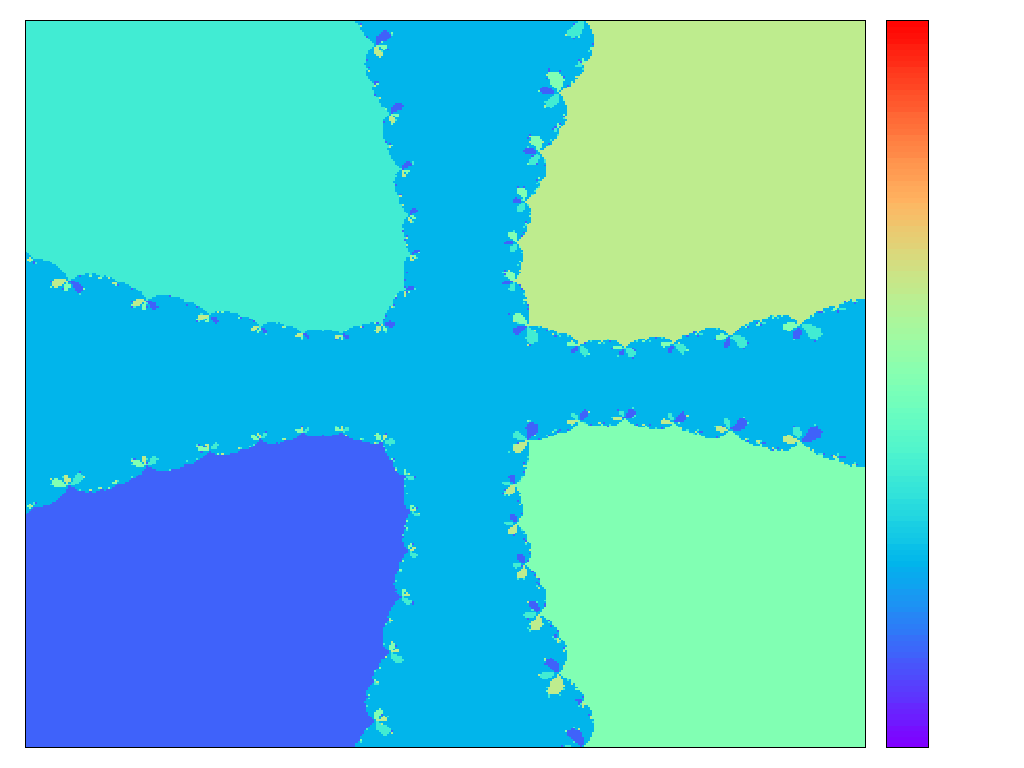
\includegraphics[scale=.4]{-9:7_7:11_3:17_0_-5_-1_400.png}

\emph{$-\frac{9}{7}x^{5} + \frac{7}{11}x^{4} + \frac{3}{17}x^{3} - 5x - 1$}

n = 400

\bigskip

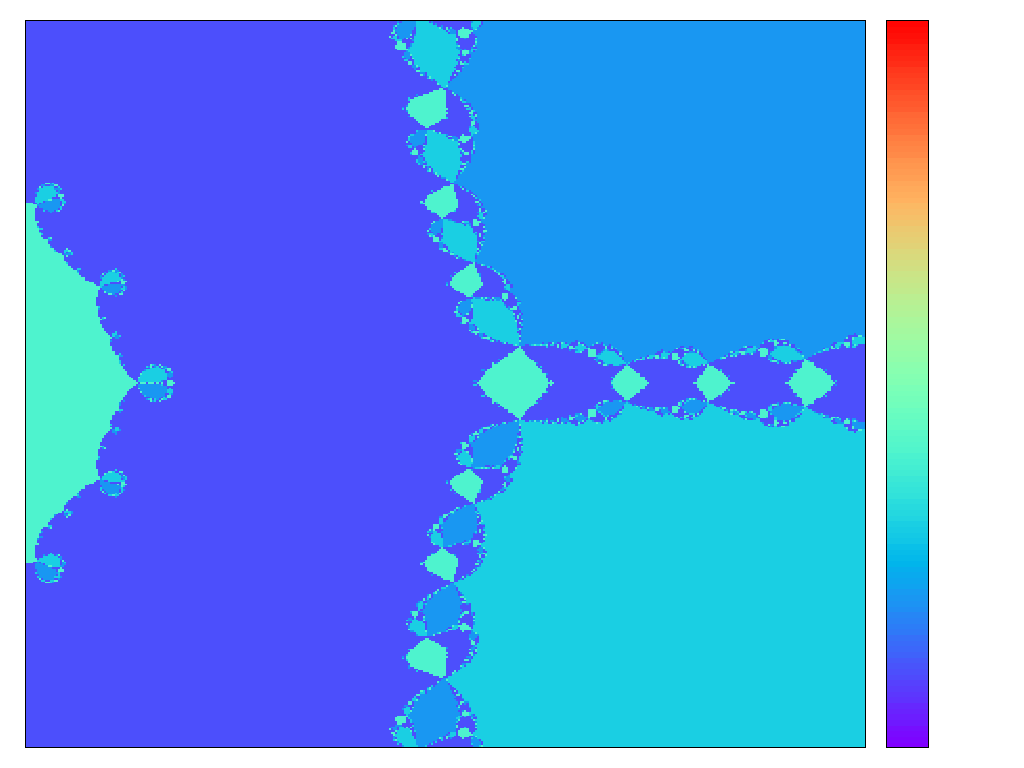
\includegraphics[scale=.4]{1_2_-7_8_12_400.png}

\emph{$x^{4} + 2x^{3} + -7x^{2} + 8 x - 12$}

n = 400

\bigskip

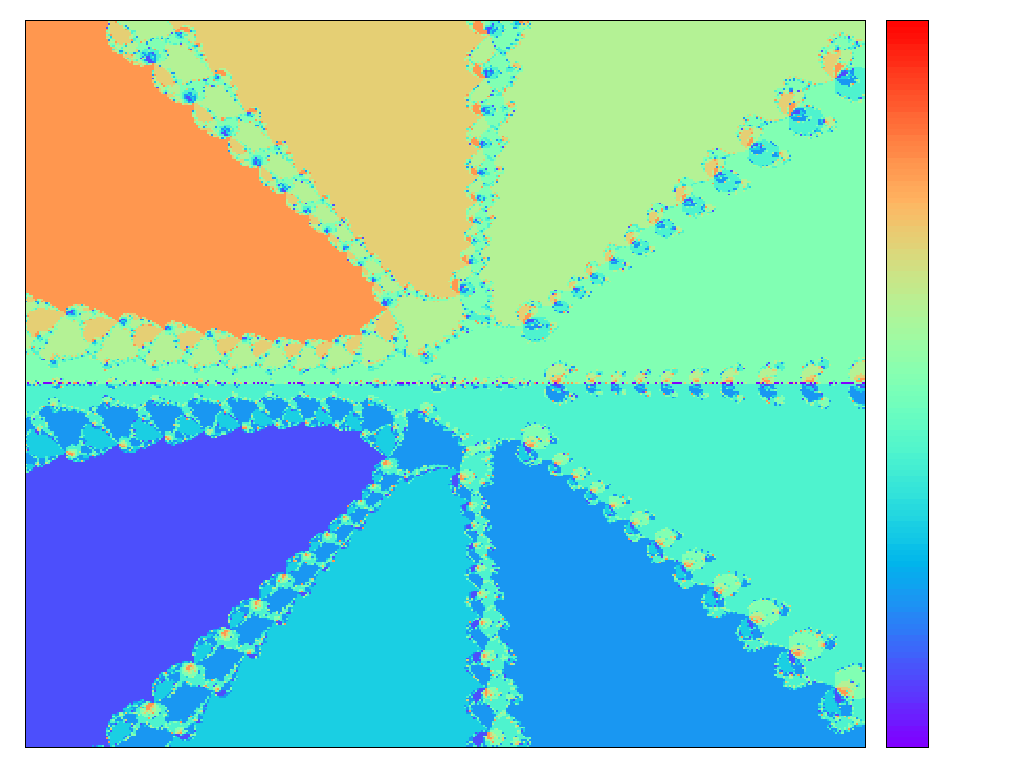
\includegraphics[scale=.4]{1_-2_3_-4_5_-6_7_-8_10_400.png}

\emph{$x^{8} + -2x^{7} + 3x^{6} - 4 x^{5} + 5x^{4} - 6x^{3} + 7x^{2} - 8x + 10$}

n = 400

\bigskip

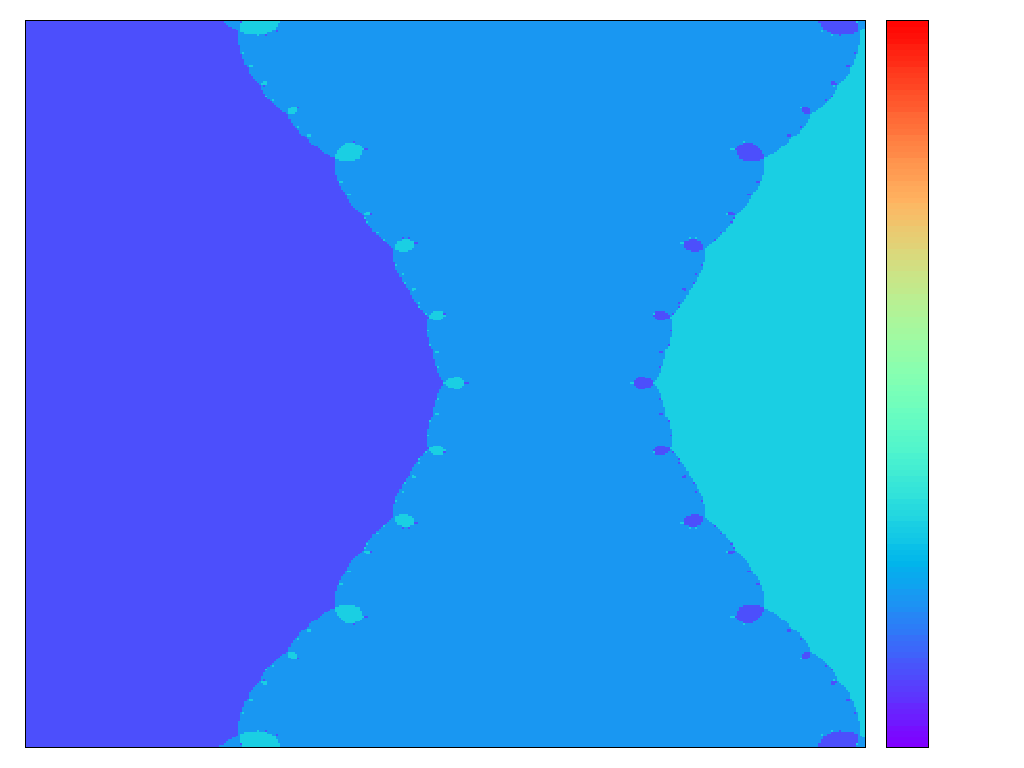
\includegraphics[scale=.4]{1_-3_0_2_400.png}

\emph{$x^{3} -3x^{2} + 2$}

n = 400

\bigskip

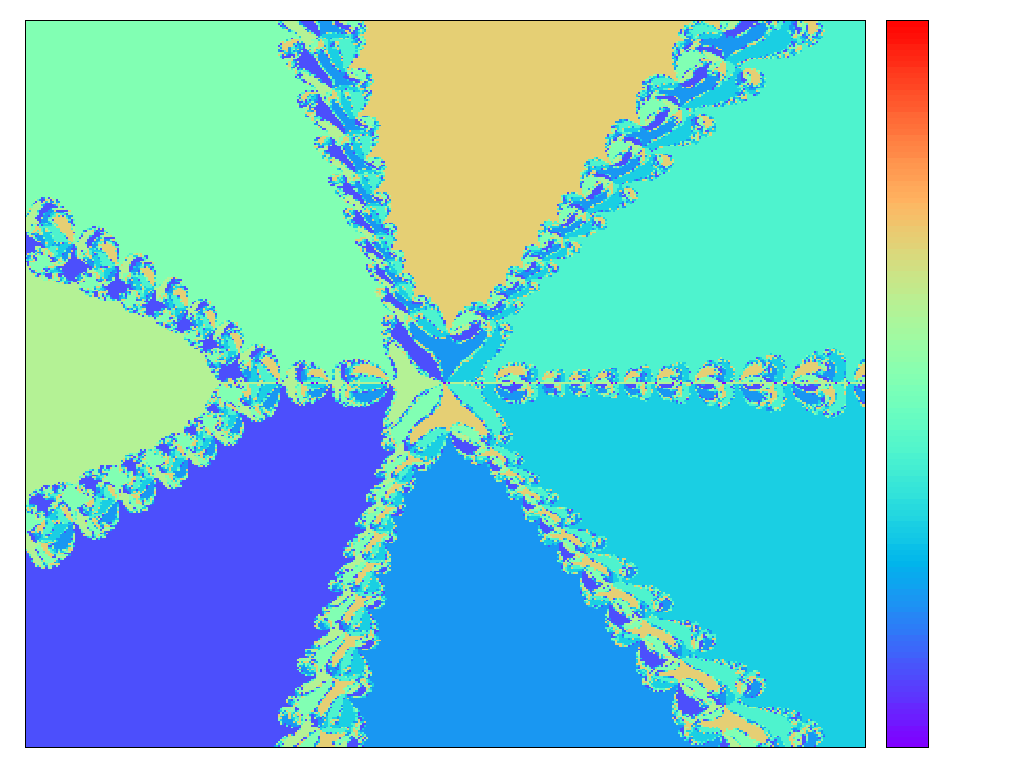
\includegraphics[scale=.4]{5_12_-3:5_7:9_0_-3_0_21_400.png}

\emph{$5x^{7} + 12x^{6} - \frac{3}{5}x^{5} + \frac{7}{9}x^{4} - 3x^{2} + 21$}

n = 400

\bigskip

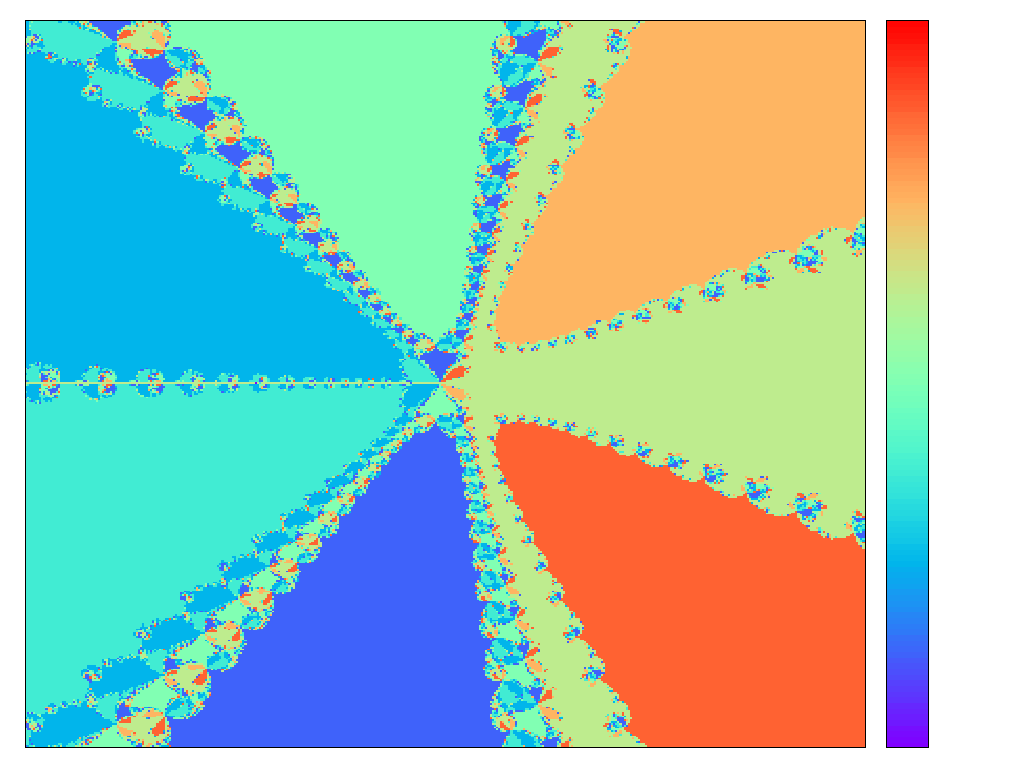
\includegraphics[scale=.4]{13_-5_0_3_1_2_1:9_-1_400.png}

\emph{$13x^{7} - 5x^{6} + 3x^{4} + x^{3} + 2x^{2} + \frac{1}{9}x - 1$}

n = 400

\end{center}

\begin{flushright}
$\blacksquare$
\end{flushright}

\section{Parte 3: Encontrando todas as raízes de uma função}

\qquad
O programa \texttt{root\_finder} não trata de casos em que há mais do que uma raíz em um subintervalo uma vez que fica por conta do usuário colocar um \texttt{ninter} pequeno o suficiente para que isso não ocorra.
 
Ele também utiliza exclusivamente o método da secante e não o de Newton uma vez que seria muito mais difícil implementar ou encontrar métodos que realizariam a derivada de funções genéricas. Isso não é um problema na segunda parte do exercício pois apenas polinômios são utilizadas nela, havendo a função \texttt{polyder()}.

No caso de não haver descrescimento suficiente como especificado pelo enunciado ($|f(x_{k})| > 0.5|f(x_{k-1})|$), a função secante retorna \texttt{NaN} como indicador de que precisa rodar o método da bissecção três vezes antes de tentar o da secante novamente.

\begin{flushright}
$\blacksquare$
\end{flushright}

\end{document}